\section{Introduction}
Schroedinger's equation for two electrons in a three-dimensional harmonic osillator well


\section{Task 02a}
Mathematical intermezzo: A unitary transformation preserves the orthogonality of the obtained eigenvectors. We assume the basis is orthogonal:
$\mathbf{v_j^Tv_i} = \delta_{ij}$

Show that an orthogonal or unitary transformation $\mathbf{w_i} = \mathbf{Uv_i}$ preserves the dot product and orthogonality, where U is a matrix.

Say $\mathbf{w_j} = \mathbf{Uv_j}$\\
\\
$\mathbf{w_j^T} = \mathbf{Uv_j}^T = \mathbf{v_j^TU^T}$\\
\\
$\mathbf{w_j^Tw_i} = \mathbf{v_j}^T \mathbf{U^TUv_i} $\\
\\
$U^TU = I \implies \mathbf{w_j^Tw_i} = \mathbf{v_j^Tv_i} = \delta_{ij}$



\section{Task 02b}
Write a function which implements Jacobi's rotation algorithm to solve the tridiagonal matrix eigenvalue problem:

The function jacobi\_method in the source code of project 2
\FloatBarrier
\begin{figure}[!ht]
\centering
\FloatBarrier
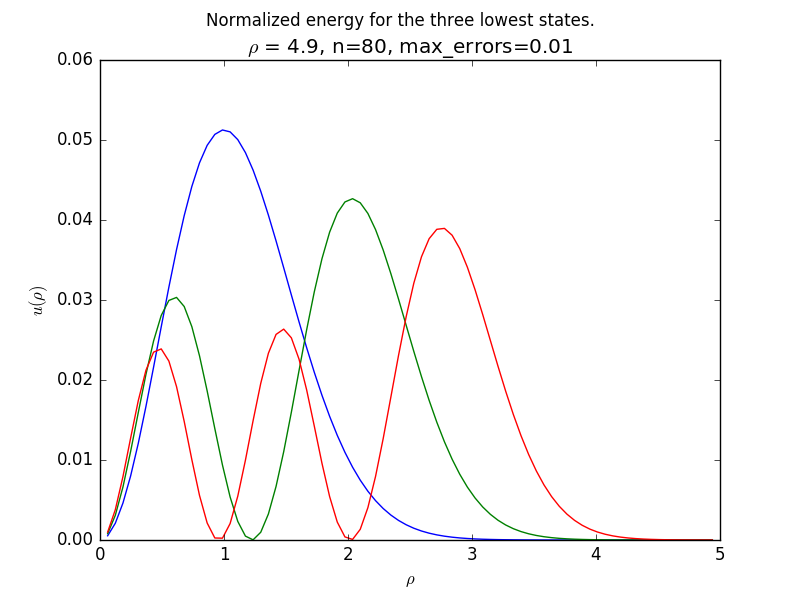
\includegraphics[width=0.45\textwidth]{eigenvector_rho49n80.png}

\caption{Computing the relative error of the numerical solution to the Poisson equation for grid sizes n =10, 100, 1000, 10000, 100000, 1000000, 10000000}
\label{fig:Error_poisson}
\end{figure}
\FloatBarrier



\FloatBarrier
\begin{figure}[!ht]
\centering
\FloatBarrier
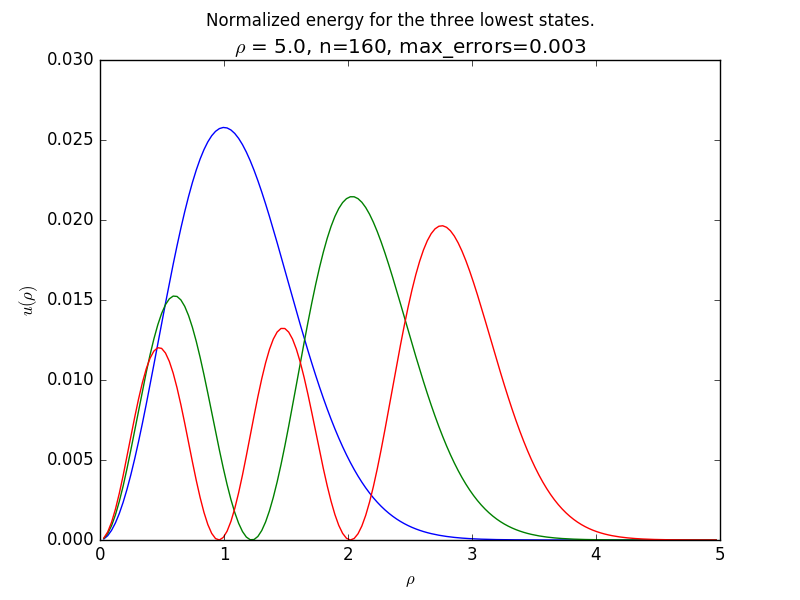
\includegraphics[width=0.45\textwidth]{eigenvector_rho49n160.png}

\caption{Computing the relative error of the numerical solution to the Poisson equation for grid sizes n =10, 100, 1000, 10000, 100000, 1000000, 10000000}
\label{fig:Error_poisson}
\end{figure}
\FloatBarrier


\FloatBarrier
\begin{figure}[!ht]
\centering
\FloatBarrier
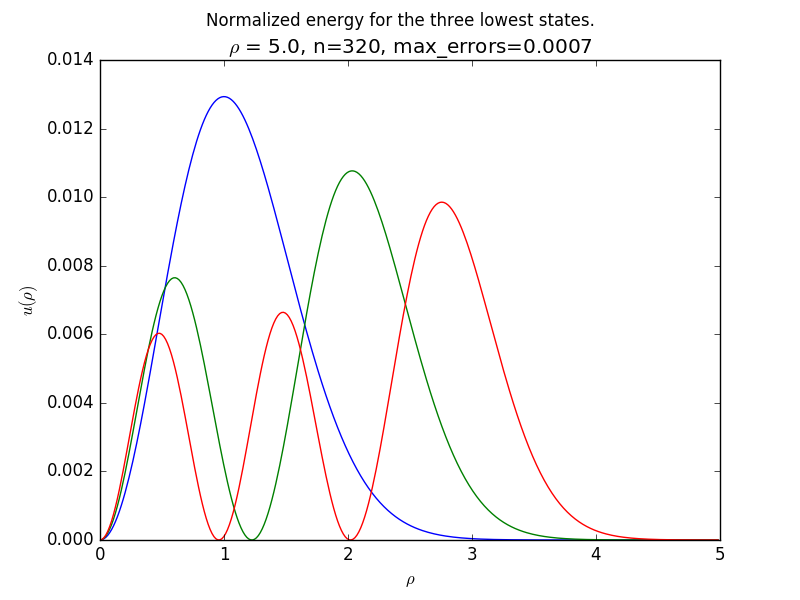
\includegraphics[width=0.45\textwidth]{eigenvector_rho49n320.png}

\caption{Computing the relative error of the numerical solution to the Poisson equation for grid sizes n =10, 100, 1000, 10000, 100000, 1000000, 10000000}
\label{fig:Error_poisson}
\end{figure}
\FloatBarrier




%\FloatBarrier
%\begin{figure}[!ht]
%\centering
%\FloatBarrier
%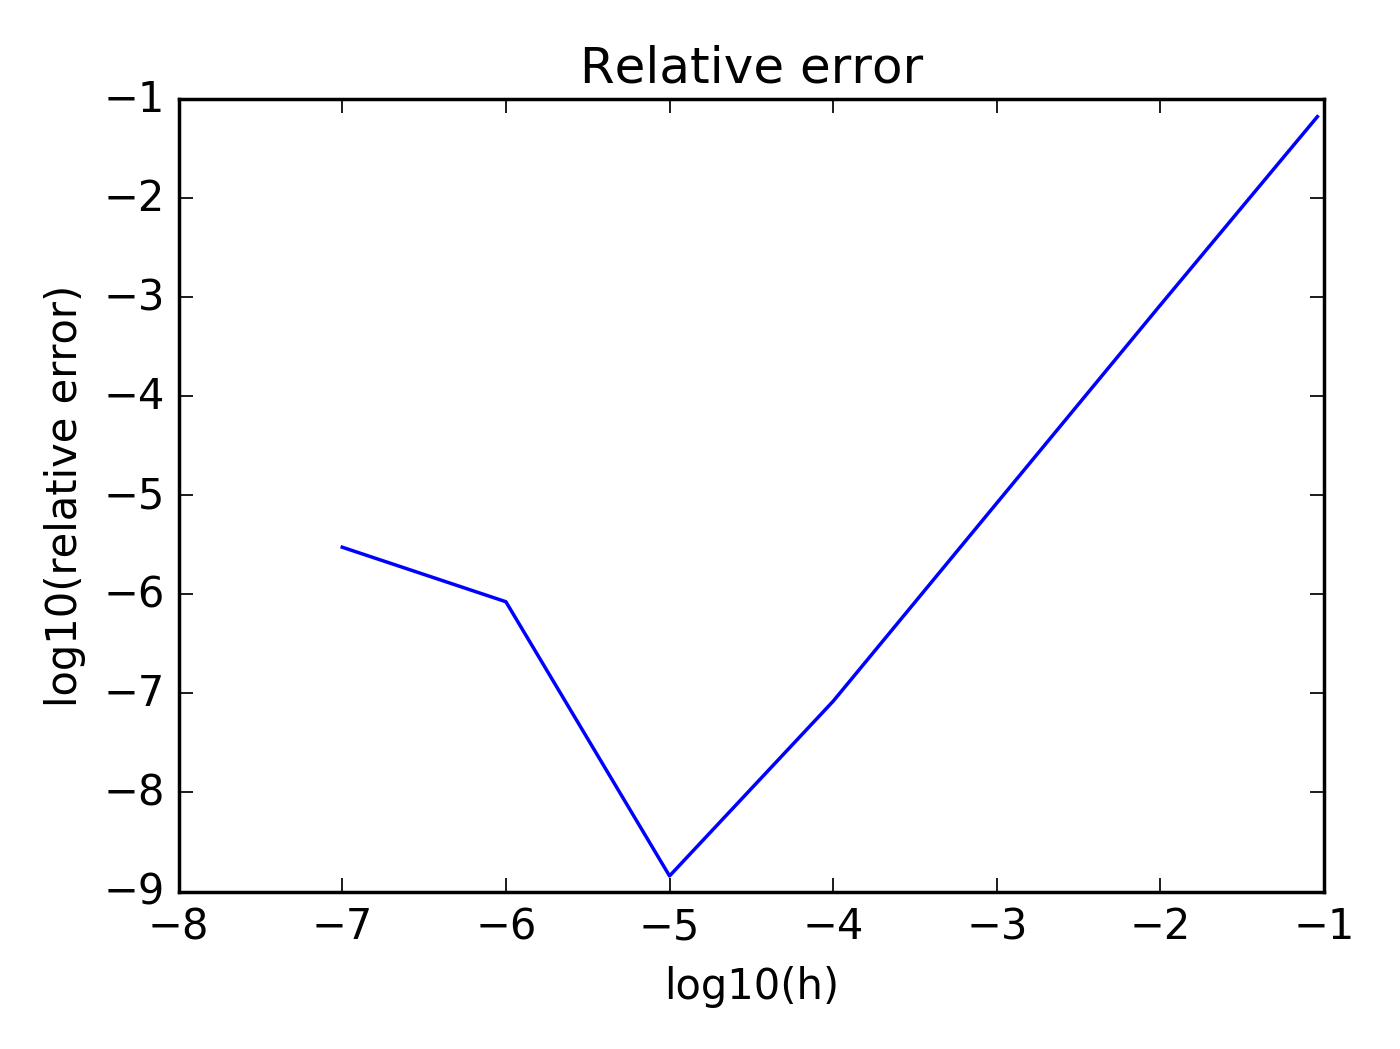
\includegraphics[width=0.45\textwidth]{error.png}
%
%\caption{Computing the relative error of the numerical solution to the Poisson equation for grid sizes n =10, 100, 1000, 10000, 100000, 1000000, 10000000}
%\label{fig:Error_poisson}
%\end{figure}
%\FloatBarrier
%
%figure~\ref{fig:Error_poisson}.\\
